\documentclass[11pt,compress]{beamer}
% deactivate beamer navigation
%\setbeamertemplate{navigation symbols}{}
%\usepackage{geometry}
%\geometry{papersize={180mm, 135mm}, top=-1.5mm} % 210mm, 297mm
\usepackage{../style/lmu-lecture}
\setbeamertemplate{frametitle}{\expandafter\uppercase\expandafter\insertframetitle}
%\useoutertheme{metropolis}
% remove section slides
\AtBeginSection[]
{
  \begin{frame}<beamer>
    \frametitle{Introduction to Machine Learning}
    \tableofcontents[currentsection]
  \end{frame}
}
% includepdf slides, pagecommad will set counter for framenumber
\usepackage{pdfpages}
\includepdfset{trim=0mm 0mm 0mm 0mm, pagecommand={\global\setcounter{framenumber}{\value{page}}}}
% trim=0mm 6mm 0mm 0mm, offset=0 15,
% add footer:
\usepackage{framed, color}
\usepackage{xcolor}
%\iffalse
\setbeamertemplate{footline}[text line]{%
    \noindent\hspace*{\dimexpr-\oddsidemargin-1in\relax}%
     \colorbox{white}{
     \makebox[\dimexpr\paperwidth-2\fboxsep\relax]{
     \color{black}
     \begin{minipage}[c][4.5ex][c]{0.5\linewidth}
       \secname
     \end{minipage}
     \hfill\begin{minipage}[c][4.5ex][c]{0.5\linewidth}
       \flushright
       \insertframenumber{}~/~\inserttotalframenumber~~
     \end{minipage}
     }}%
  \hspace*{-\paperwidth}
}
%\fi

\begin{document}
\setbeamercolor{background canvas}{bg=}

% General remark: hyperlinks in included pdfs are not clickable anymore in the combined pd

\section{Performance Evaluation} %60min.?

\includepdf[pages={1-last}]{slides-evaluation-intro.pdf}
%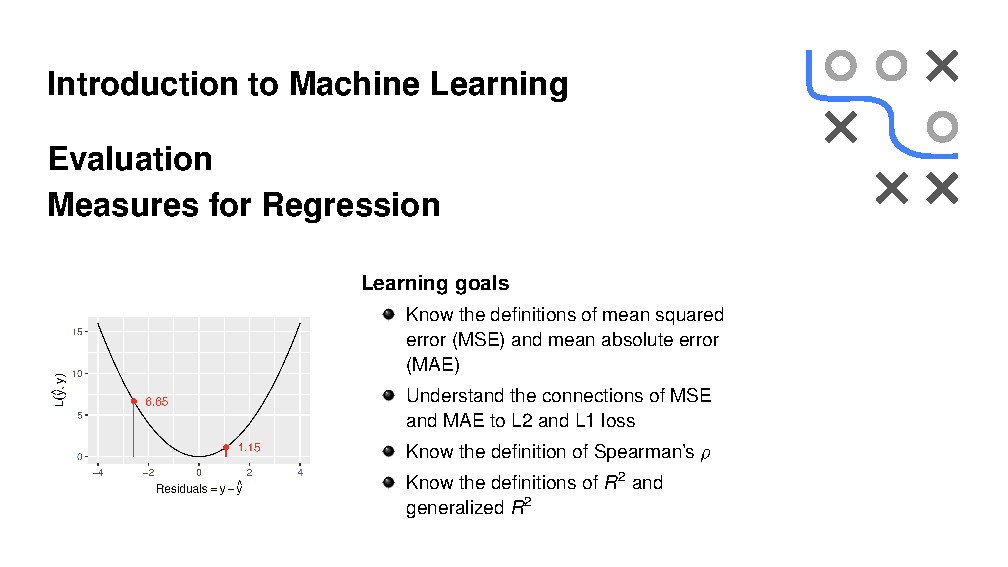
\includepdf[pages={1-4}]{slides-evaluation-measures-regression.pdf}
%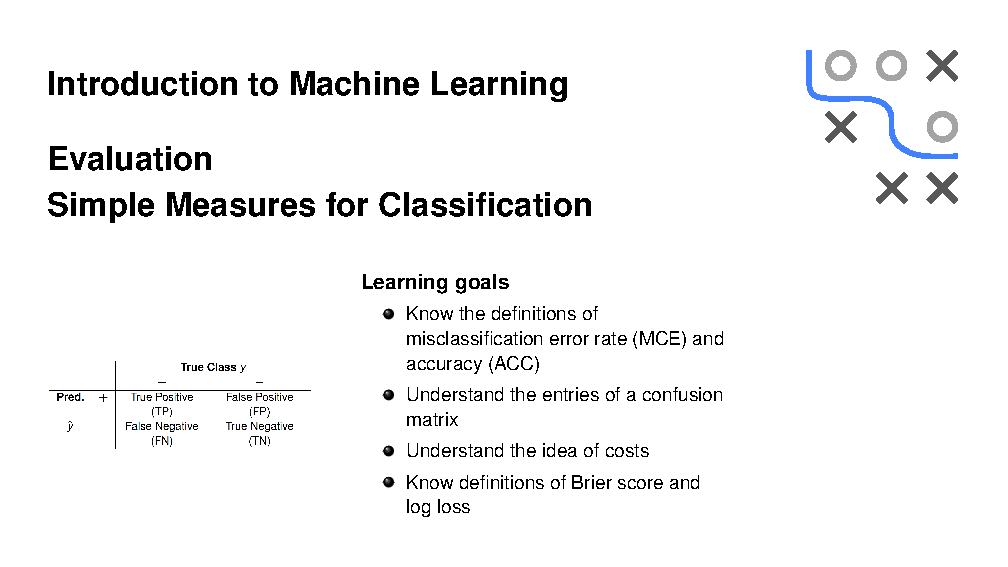
\includepdf[pages={1-5, 8-last}]{slides-evaluation-measures-classification.pdf}
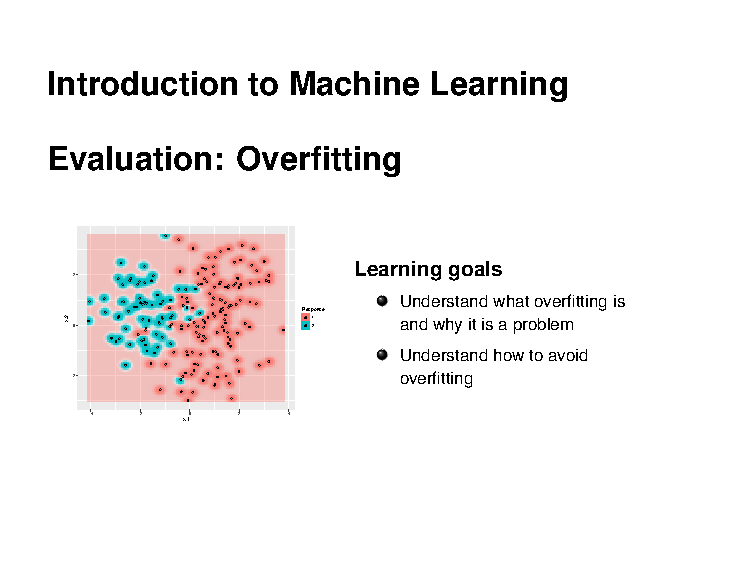
\includepdf[pages={1-last}]{slides-evaluation-overfitting.pdf}
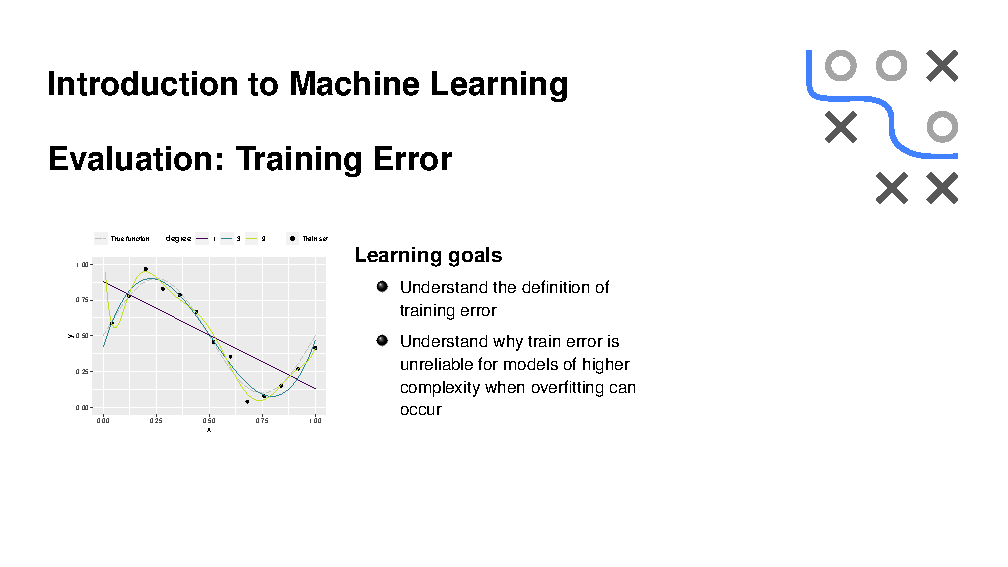
\includepdf[pages={1-last}]{slides-evaluation-train.pdf}

\includepdf[pages={1-last}]{slides-evaluation-test.pdf}

\includepdf[pages={1-last}]{slides-evaluation-resampling.pdf}

\section{Random Forests} %60min.?
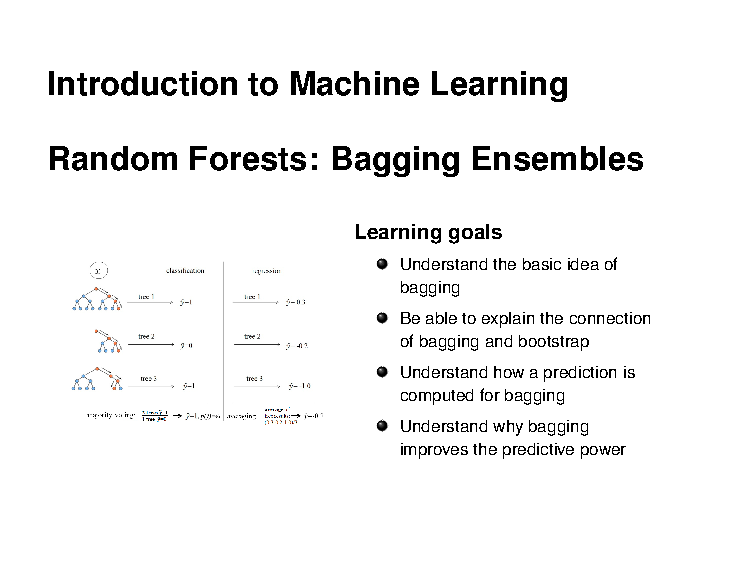
\includepdf[pages={1-4}]{slides-forests-bagging.pdf}
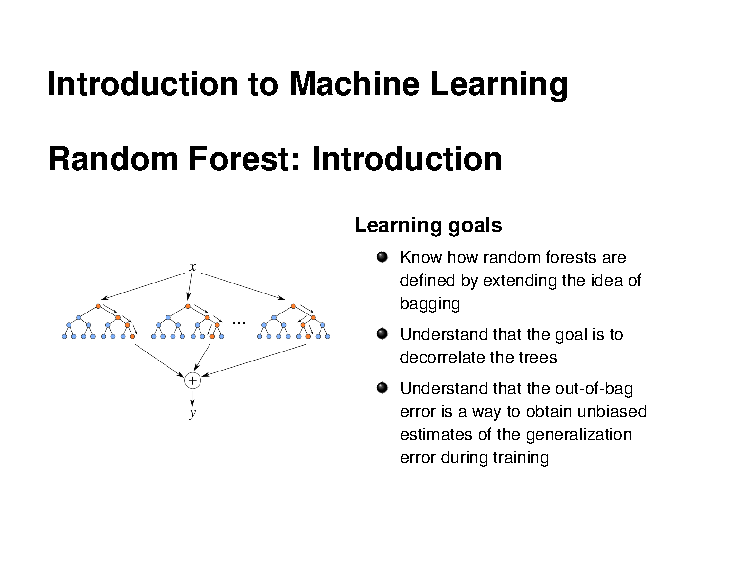
\includepdf[pages={1-last}]{slides-forests-intro.pdf}
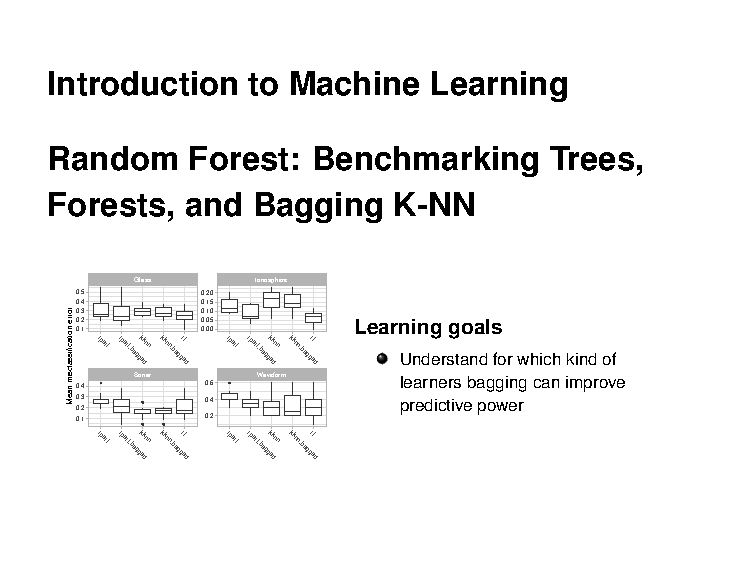
\includepdf[pages={1-last}]{slides-forests-benchmark.pdf}
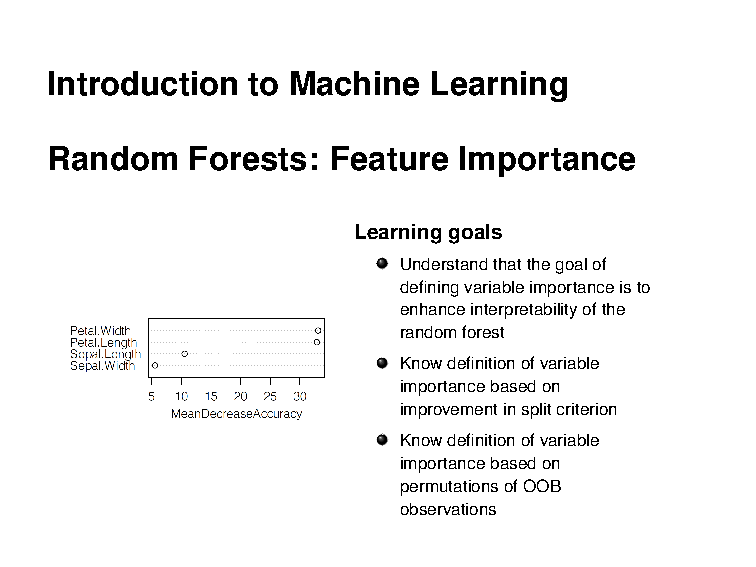
\includepdf[pages={1-last}]{slides-forests-featureimportance.pdf}
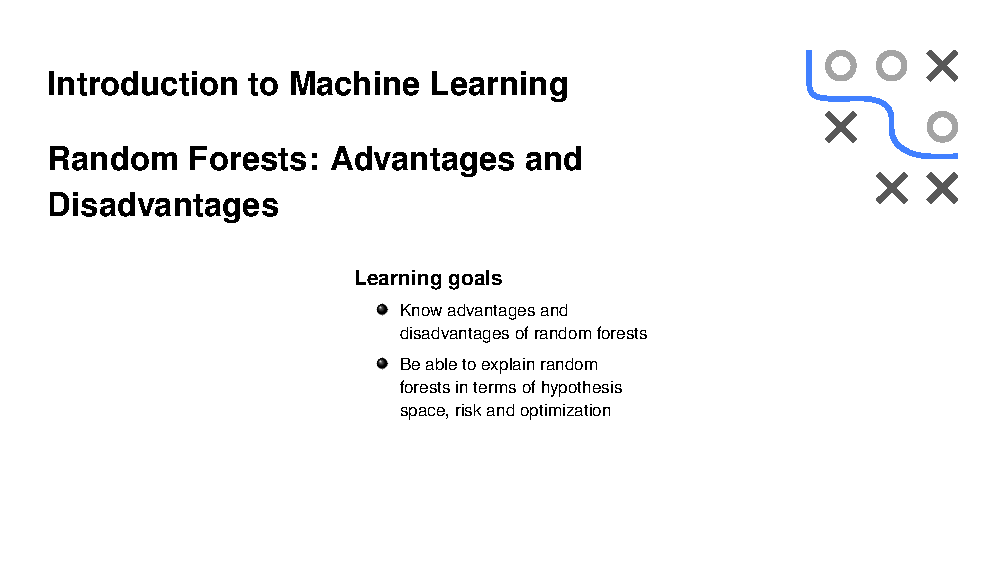
\includepdf[pages={1-last}]{slides-forests-discussion.pdf}

\section{mlr3 Resampling} %30min. (inkl. use case demo continuing from resampling)?
\includepdf[pages={2-last}]{../slides/mlr3/slides-mlr3-resampling.pdf}

\section{Exercise: mlr3 Resampling} %60min. (hands-on exercise)?
\begin{frame}{Exercise: mlr3 Resampling}
\begin{enumerate}
\item Evaluate the performance of a learner on the \texttt{iris} data set using the classification error as performance measure and 5-fold cross-validation for resampling.
\item Use the \textbf{benchmark} function to compare your learner against another learner using the classification error as performance measure and 5-fold cross-validation for resampling.
\item Bonus Exercise: Re-run the previous benchmark and use the classification error (CE) \textbf{and} the prediction accuracy (ACC) as performance measure (see \texttt{as.data.table(mlr\_measures)}).
%\textbf{and} the area under the ROC curve (AUC)  Hint: You may need to remember how to configure a learner to predict \href{https://mlr3gallery.mlr-org.com/posts/2020-03-11-basics-german-credit/\#predict-probabilities}{\underline{probabilities}.}
\end{enumerate}
\end{frame}

\section{Tuning} % 30 min.
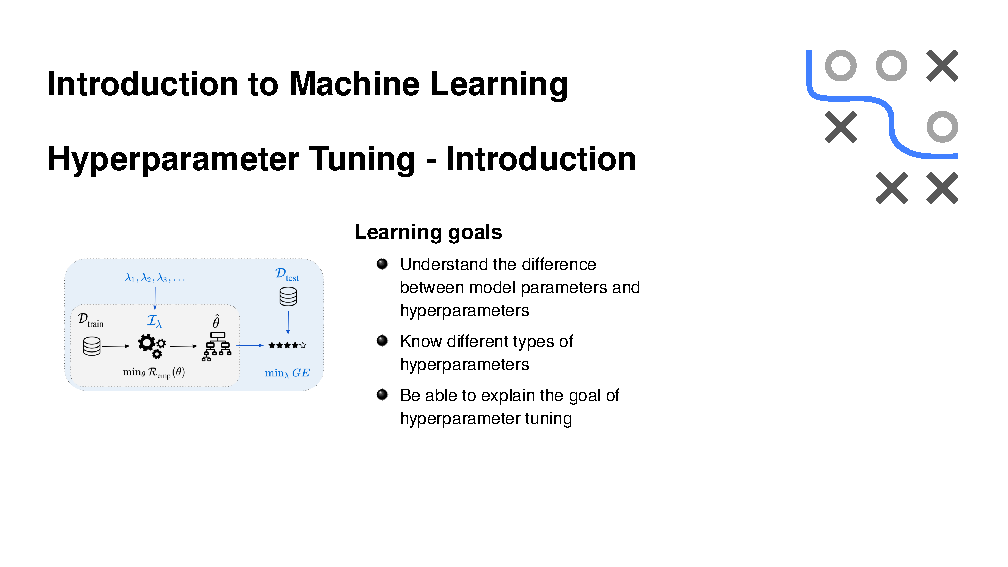
\includepdf[pages={1-last}]{slides-tuning-intro.pdf}
\includepdf[pages={2-3, 6-last}]{slides-tuning-tuningproblem.pdf}
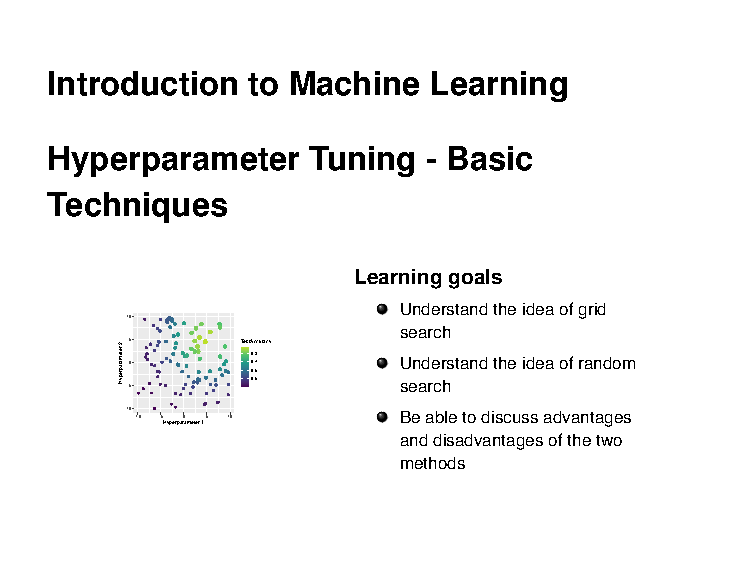
\includepdf[pages={1-last}]{slides-tuning-basicalgos.pdf}

\section{Tuning with mlr3tuning} % 30 min.

\includepdf[pages={6-8, 12-35, 38-40, 43-53, 57, 62-69}]{../slides/mlr3/slides-mlr3-tuning.pdf}

\section{Exercise: Tuning with mlr3tuning}
\begin{frame}{Exercise: Tuning with mlr3tuning}
\begin{itemize}
\item \textbf{Demo:} \newline\href{https://mlr3gallery.mlr-org.com/posts/2020-03-11-mlr3tuning-tutorial-german-credit/}{\underline{mlr3tuning Tutorial}} (Stop at Section Nested Resampling)
\item \textbf{Exercise:} Modify the previous demo on the \textbf{german credit} data according to the following exercises.
\begin{enumerate}
%\item To tune a random forest (\texttt{ranger}) and find the best hyperparameters for \texttt{mtry}, \texttt{min.node.size}, and \texttt{replace} via \textbf{random search}. See \texttt{?ranger} for a description of the hyperparameters.
\item Tune a decision tree (\texttt{rpart}) and specify the search space for \texttt{minsplit} (from 1 to 200) and \texttt{maxdepth} (from 10 to 30). Use 50 evaluations as termination criterion, the classification error \texttt{msr("classif.ce")} as performance measure, and 3-fold CV as resampling strategy.
\item Visualize the results using ggplot to see how \texttt{minsplit} and \texttt{maxdepth} affect the performance.
\item Optional: Change your previous code and use the brier score \texttt{msr("classif.bbrier")} as performance measure instead of the classification error for tuning (hint: You need to modify your learner such that it predicts probabilites).
\end{enumerate}
\end{itemize}
\end{frame}
\end{document}
